\subsection{Functions of Multiple Variables}

\begin{example}
$f(x,y) = \sqrt{(x+1)(y-2)}$, \; implied domain: $(x+1)(y-2)\ge 0$.
\end{example}

Graph of $f(x,y)$ is the set of points $(x,\,y,\,f(x,y))$.

\begin{example}[$f(x,y)=x^{2}+y^{2}$]
Implied domain $\R^{2}$.
\begin{itemize}
    \item Horizontal cross sections: $z = x^{2}+y^{2} = \text{const}$ — circles
    \item Vertical cross sections: $x = \text{const}$ — parabola
\end{itemize}

\begin{center}
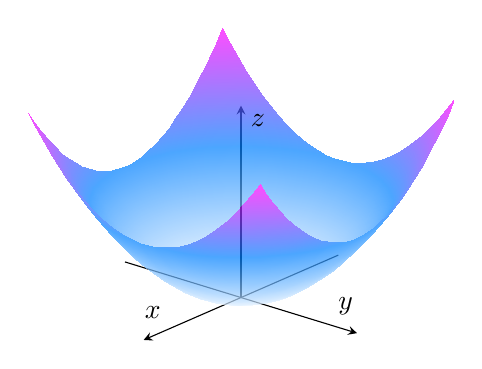
\begin{tikzpicture}
    \begin{axis}[
        view={130}{30}, width=7cm, height=6cm,
        xlabel=$x$, ylabel=$y$, zlabel=$z$,
        domain=-1.5:1.5, y domain=-1.5:1.5,
        samples=30, colormap/cool,
        axis lines=center, ticks=none,
    ]
    \addplot3[surf, opacity=0.7, shader=interp]{x^2+y^2};
    \end{axis}
\end{tikzpicture}
\end{center}
\end{example}

Curves where $x$/$y$/$z = \text{const}$ are called \textbf{level curves} (or contours).

\begin{example}
$f(x,y,z)=x^{2}+y^{2}+z^{2}$. \;
$f(x,y,z)=k$ gives level surfaces: concentric spheres.
\end{example}

\subsection{Limits and Continuity}

\begin{definition}[Limit]
$\displaystyle\lim_{(x,y)\to(a,b)}f(x,y) = L$:
as $(x,y)$ approaches $(a,b)$, $f(x,y)$ tends to $L$.

Formally (when $L\neq\pm\infty$):
\[
    \forall\,\varepsilon>0,\;\exists\,\delta>0
    \text{ such that }
    \lvert(x,y)-(a,b)\rvert<\delta
    \;\Longrightarrow\;
    \lvert f(x,y)-L\rvert<\varepsilon
\]
\end{definition}

\begin{definition}[Continuity]
$f(x,y)$ continuous at $(a,b)$
$\;\Longleftrightarrow\;$
$\displaystyle\lim_{(x,y)\to(a,b)}f(x,y) = f(a,b)$.
\end{definition}

\begin{example}
\[
    f(x,y) =
    \begin{cases}
        \dfrac{xy}{x^{2}+y^{2}} & (x,y)\neq(0,0) \\[6pt]
        0 & \text{else}
    \end{cases}
\]
Is $f$ continuous at $(0,0)$?

Suppose $f$ is continuous at $(0,0)$.
Take any sequence $(x_{n},y_{n})\to(0,0)$:
\[
    \lim_{n\to\infty}f(x_{n},y_{n}) = 0 = f(0,0)
\]

$1^{\circ}$ Let $(x_{n},y_{n})=\bigl(0,\tfrac{1}{n}\bigr)\to(0,0)$:
\[
    \lim_{n\to\infty}f(x_{n},y_{n})
    = \lim_{n\to\infty}\frac{0}{0+1/n^{2}} = 0
\]

$2^{\circ}$ Let $(x_{n},y_{n})=\bigl(\tfrac{1}{n},\tfrac{1}{n}\bigr)\to(0,0)$:
\[
    \lim_{n\to\infty}f(x_{n},y_{n})
    = \lim_{n\to\infty}\frac{1/n^{2}}{2/n^{2}} = \frac{1}{2}
\]

Contradictory. Limit does not exist $\;\Longrightarrow\;$ not continuous.
\end{example}

\begin{example}
\[
    \lim_{(x,y)\to(0,0)}\frac{x-y}{y-\ln(1+x)} \;=\; ?
\]
Let $y=kx$:
\[
    f(x,kx) = \frac{x-kx}{kx-\ln(1+x)}
\]
Apply L'H\^{o}pital's rule as $x\to 0$:
\[
    \lim_{x\to 0}\frac{1-k}{k-\dfrac{1}{1+x}} = \frac{1-k}{k-1} = -1
\]
When $k=1$: $\displaystyle\lim = 0$. \; Contradiction $\Longrightarrow$ limit does not exist.
\end{example}

\subsection{Partial Derivatives}

\begin{definition}[Partial derivative]
Given $f(x,y)$, let $y=$ constant $b$ $\;\Longrightarrow\;$ $g(x)=f(x,b)$.
\[
    \frac{dg}{dx} = \pd{f}{x}\bigg|_{(x,b)} = f_{x}(x,b)
\]
Partial derivative of $f$ with respect to $x$: treat all other variables as constants.

Formally:
\[
    \pd{f}{x} = \lim_{h\to 0}\frac{f(x+h,y)-f(x,y)}{h}
\]
\end{definition}

\begin{example}
$f(x,y) = x^{2}+xy^{3}$
\[
    \pd{f}{x} = 2x+y^{3}
    \qquad
    \pd{f}{y} = 3xy^{2}
\]
\end{example}

\begin{example}
$f(x,y) = \cos(x^{3}y)+e^{xy}$
\[
    \pd{f}{x}
    = -\sin(x^{3}y)\cdot 3x^{2}y + e^{xy}\cdot y
\]
\end{example}

\begin{example}
$f(x,y,z) = x^{yz}$. \; Write $f = e^{yz\ln x}$:
\[
    \pd{f}{x} = yz\,x^{yz-1}
    \qquad
    \pd{f}{y} = z\ln x\cdot x^{yz}
\]
\end{example}

\subsubsection*{Higher Order Derivatives}

\[
    f_{xx} = \frac{\partial^{2}f}{\partial x^{2}}, \qquad
    f_{yy} = \frac{\partial^{2}f}{\partial y^{2}}, \qquad
    f_{xy} = \frac{\partial^{2}f}{\partial y\,\partial x}, \qquad
    f_{yx} = \frac{\partial^{2}f}{\partial x\,\partial y}
\]

\begin{theorem}[Clairaut's]
$f_{xy}=f_{yx}$ — mixed partial derivatives commute (when both are continuous).
\end{theorem}

\subsubsection*{Approximation}

\[
    f(x+h,\,y) \approx f(x,y) + h\,\pd{f}{x}
\]

\subsubsection*{Partial Differential Equations (PDE)}

Differential equations with partial derivatives.

\begin{example}[Laplace equation]
$u(x,y)$: \; $u_{xx}+u_{yy}=0$
\end{example}

\subsubsection*{Implicit Partial Derivatives}

\begin{example}
Particle on surface $x^{2}+y^{2}+xyz^{2}=3$, at $(1,1,1)$.
Suppose $\Delta x=\tfrac{1}{10}$, $\Delta y=-\tfrac{1}{5}$.
Find approx change in $z$.

Differentiate both sides w.r.t.\ $x$:
$\;\pd{}{x}(\text{LHS}) = \pd{}{x}(\text{RHS})$.
\[
    2x\dd{x}+2y\dd{y}+yz^{2}\dd{x}+xz^{2}\dd{y}+2xyz\dd{z}=0
\]
Plug in $(1,1,1)$:
\[
    3\dd{x}+3\dd{y}+2\dd{z}=0
\]
Approximate: $3\bigl(\tfrac{1}{10}\bigr)+3\bigl(-\tfrac{1}{5}\bigr)+2\,\Delta z=0
\;\Longrightarrow\;
\Delta z = \dfrac{3}{20}$
\end{example}

\subsection{Tangent Planes and Linear Approximations}

Recall single variable: tangent line at $(x_{0},y_{0})$:
\[
    L\colon y-y_{0} = f'(x_{0})(x-x_{0})
\]

Other perspective: $\mathbf{r}(t)=\begin{pmatrix}t\\f(t)\end{pmatrix}$, \;
tangent vector $\mathbf{r}'=\begin{pmatrix}1\\f'(t)\end{pmatrix}$.

Tangent line:
$\begin{pmatrix}x\\y\end{pmatrix}
= \begin{pmatrix}x_{0}\\y_{0}\end{pmatrix}
+ \lambda\begin{pmatrix}1\\f'(x_{0})\end{pmatrix}$
— passes through $P$, parallel to tangent vector.

\begin{definition}[Tangent plane]
Tangent plane to surface $z=f(x,y)$ at $P(x_{0},y_{0},z_{0})$:
\[
    z = z_{0} + f_{x}(x_{0},y_{0})(x-x_{0}) + f_{y}(x_{0},y_{0})(y-y_{0})
\]
\end{definition}

\begin{example}
$z = x^{2}+y^{4}$ at $P(2,1,5)$. \;
$f_{x}=2x$, $f_{y}=4y^{3}$.
\[
    z = 5+4(x-2)+4(y-1) = 4x+4y-7
\]
\end{example}

\subsubsection*{Why a plane?}

Parametrize $z=f(x,y)$:
$\mathbf{r}(x,y)=\begin{pmatrix}x\\y\\f(x,y)\end{pmatrix}$.

\[
    \mathbf{u} = \pd{\mathbf{r}}{x}=\begin{pmatrix}1\\0\\f_{x}\end{pmatrix},
    \qquad
    \mathbf{v} = \pd{\mathbf{r}}{y}=\begin{pmatrix}0\\1\\f_{y}\end{pmatrix}
\]

Normal vector:
$\mathbf{n}=\mathbf{u}\times\mathbf{v}=\begin{pmatrix}-f_{x}\\-f_{y}\\1\end{pmatrix}$

\[
    0 = (\mathbf{x}-\mathbf{x}_{0})\cdot\mathbf{n}
    \;\Longrightarrow\;
    0 = -f_{x}(x-x_{0})-f_{y}(y-y_{0})+(z-z_{0})
\]

\begin{definition}[Linear approximation]
$f(x_{0}+\Delta x,\,y_{0}+\Delta y)
\approx f(x_{0},y_{0})+f_{x}(Q)\,\Delta x+f_{y}(Q)\,\Delta y$

Total differential: $dz = f_{x}\dd{x}+f_{y}\dd{y}$
\end{definition}

\subsection{The Chain Rule}

Recall single variable:
$\dfrac{d}{dx}f(g(x))=f'(g(x))\,g'(x)=\dfrac{df}{dg}\,\dfrac{dg}{dx}$

\begin{theorem}
If $f(x,y)$ is differentiable and $x(t)$, $y(t)$ are differentiable, then
$f(x(t),y(t))$ is differentiable w.r.t.\ $t$:
\[
    \frac{df}{dt}
    = \pd{f}{x}\,\frac{dx}{dt}+\pd{f}{y}\,\frac{dy}{dt}
\]
\end{theorem}

\begin{example}
$f(x,y)=x^{2}+3xy$, \; $x(t)=2t$, \; $y(t)=\sqrt{t}$.

$\pd{f}{x}=2x+3y$, \; $\pd{f}{y}=3x$, \;
$\dfrac{dx}{dt}=2$, \; $\dfrac{dy}{dt}=\dfrac{1}{2}t^{-1/2}$

\begin{align*}
    \frac{d}{dt}f(x(t),y(t))
    &= (2x+3y)\cdot 2 + 3x\cdot\tfrac{1}{2}t^{-1/2} \\
    &= (4t+3\sqrt{t})\cdot 2 + 3(2t)\cdot\tfrac{1}{2}t^{-1/2} \\
    &= 8t+6\sqrt{t}+3\sqrt{t} \\
    &= 8t+9\sqrt{t}
\end{align*}
\end{example}

\begin{theorem}[Chain rule — two intermediate variables]
If $f(x,y)$ is differentiable and $x(s,t)$, $y(s,t)$ are differentiable,
then $f(x(s,t),y(s,t))$ is differentiable w.r.t.\ $s$ and $t$:
\[
    \pd{f}{s} = \pd{f}{x}\,\pd{x}{s}+\pd{f}{y}\,\pd{y}{s},
    \qquad
    \pd{f}{t} = \pd{f}{x}\,\pd{x}{t}+\pd{f}{y}\,\pd{y}{t}
\]
\end{theorem}

\begin{example}
$f(x,y)=x^{2}y$. Put $f$ into polar coordinates, then find $\pd{f}{\theta}$.

\[
    \pd{f}{\theta}
    = \pd{f}{x}\,\pd{x}{\theta}+\pd{f}{y}\,\pd{y}{\theta}
    = 2xy\cdot(-r\sin\theta)+x^{2}\cdot r\cos\theta
    = -2r^{3}\cos\theta\sin^{2}\theta+r^{3}\cos^{3}\theta
\]
\end{example}

\begin{example}[Polar $\leftrightarrow$ Cartesian partials]
Given $f(\theta,r)$ and $f(x,y)$ with
$r=\sqrt{x^{2}+y^{2}}$, $\theta=\arctan\dfrac{y}{x}$:
\[
    \pd{f}{x} = \cos\theta\,\pd{f}{r}-\frac{\sin\theta}{r}\,\pd{f}{\theta},
    \qquad
    \pd{f}{y} = \sin\theta\,\pd{f}{r}+\frac{\cos\theta}{r}\,\pd{f}{\theta}
\]

Solving for $\pd{f}{\theta}$:
multiply $\pd{f}{y}$ by $\cos\theta$ and $\pd{f}{x}$ by $(-\sin\theta)$, then add:
\[
    \pd{f}{\theta}
    = r\cos\theta\,\pd{f}{y}-r\sin\theta\,\pd{f}{x}
    = x\,\pd{f}{y}-y\,\pd{f}{x}
\]
\end{example}

\subsection{Directional Derivatives and the Gradient}

Take a tiny step from $P=(x_{0},y_{0})$ in direction
$\hat{\mathbf{u}}=\begin{pmatrix}a\\b\end{pmatrix}$ (unit vector)
for a function $f(x,y)$.

\begin{center}
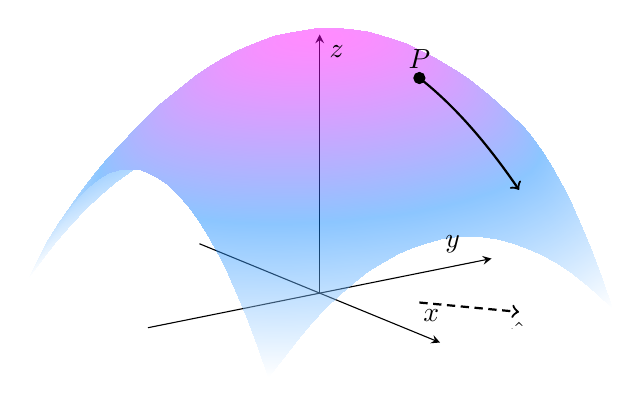
\begin{tikzpicture}
    \begin{axis}[
        view={55}{25}, width=9cm, height=7cm,
        xlabel=$x$, ylabel=$y$, zlabel=$z$,
        domain=-2:2, y domain=-2:2,
        samples=25, colormap/cool,
        axis lines=center, ticks=none,
    ]
    % surface z = 2 - 0.3x^2 - 0.2y^2
    \addplot3[surf, opacity=0.45, shader=interp]{2-0.3*x^2-0.2*y^2};
    % point P on surface
    \addplot3[only marks, mark=*, mark size=2pt] coordinates {(0.8,0.6,{2-0.3*0.64-0.2*0.36})};
    \node at (axis cs:0.8,0.6,{2-0.3*0.64-0.2*0.36+0.15}) {$P$};
    % direction vector u in the xy-plane
    \draw[->, thick, densely dashed] (axis cs:0.8,0.6,0) -- (axis cs:1.6,1.2,0)
        node[below]{$\hat{\mathbf{u}}$};
    % slope line on surface in direction u
    \addplot3[thick, ->, domain=0:1, samples=20, samples y=0]
        ({0.8+0.8*x},{0.6+0.6*x},{2-0.3*(0.8+0.8*x)^2-0.2*(0.6+0.6*x)^2});
    \end{axis}
\end{tikzpicture}
\end{center}

\begin{definition}[Directional derivative]
\[
    D_{\hat{\mathbf{u}}}\,f(x_{0},y_{0})
    = \lim_{h\to 0}\frac{f(x_{0}+ha,\,y_{0}+hb)-f(x_{0},y_{0})}{h}
    = a\,f_{x}+b\,f_{y}
    = \hat{\mathbf{u}}\cdot\begin{pmatrix}f_{x}\\f_{y}\end{pmatrix}
\]
\end{definition}

\begin{example}
$f(x,y)=x^{2}y+3xy^{3}$, \;
$\hat{\mathbf{u}}=\begin{pmatrix}4/5\\3/5\end{pmatrix}$, \;
$P=(1,2)$.
\[
    D_{\hat{\mathbf{u}}}f(P)
    = \tfrac{4}{5}\,\pd{f}{x}\bigg|_{P}+\tfrac{3}{5}\,\pd{f}{y}\bigg|_{P}
    = \tfrac{4}{5}(2xy+3y^{3})\big|_{P}+\tfrac{3}{5}(x^{2}+9xy^{2})\big|_{P}
\]
\end{example}

\begin{definition}[Gradient]
The gradient of $f(x,y)$ is
\[
    \nabla f = \begin{pmatrix}f_{x}\\f_{y}\end{pmatrix}
    \qquad (\R^{2}\mapsto\R^{2})
\]
Pronounced ``grad $f$'' or ``nabla $f$''.
\end{definition}

\begin{example}
$f(x,y)=x^{3}\cos(xy)$.
\[
    \nabla f
    = \begin{pmatrix}3x^{2}\cos(xy)-x^{3}y\sin(xy)\\-x^{4}\sin(xy)\end{pmatrix}
\]
At $P=(\pi/2,\,1)$, the directional derivative in direction
$\hat{\mathbf{u}}=\begin{pmatrix}12/13\\5/13\end{pmatrix}$:
\[
    D_{\hat{\mathbf{u}}}f(P) = \hat{\mathbf{u}}\cdot\nabla f(P)
    = \begin{pmatrix}12/13\\5/13\end{pmatrix}\cdot
      \begin{pmatrix}-(\pi/2)^{3}\\-(\pi/2)^{4}\end{pmatrix}
\]
\end{example}

\subsubsection*{Geometric Interpretation}

All unit vectors can be written as
$\hat{\mathbf{u}}=\begin{pmatrix}\cos\phi\\\sin\phi\end{pmatrix}$, so
\[
    D_{\hat{\mathbf{u}}}f = \cos\phi\,f_{x}+\sin\phi\,f_{y}
    = \hat{\mathbf{u}}\cdot\nabla f
    = \lVert\nabla f\rVert\cos\theta
\]
where $\theta=\angle(\hat{\mathbf{u}},\nabla f)$.

\begin{itemize}
    \item $D_{\hat{\mathbf{u}}}f$ is \textbf{max} at $\theta=0$:
          $\hat{\mathbf{u}}\parallel\nabla f$,
          value $=\lVert\nabla f\rVert$
    \item $D_{\hat{\mathbf{u}}}f$ is \textbf{min} at $\theta=180^{\circ}$:
          value $=-\lVert\nabla f\rVert$
    \item $D_{\hat{\mathbf{u}}}f=0$ at $\theta=90^{\circ}$:
          $\hat{\mathbf{u}}\perp\nabla f$
          $\;\Longleftrightarrow\;$
          $\tan\phi=-f_{x}/f_{y}$
\end{itemize}

At any point on a surface, there are directions $\phi$, $\phi+\pi$ for which $D_{\hat{\mathbf{u}}}f=0$.

\subsubsection*{Higher Dimensions}

$\nabla f = \ve{f_{x_{1}},\,f_{x_{2}},\,\dots,\,f_{x_{n}}}$, \;
$\R^{n}\mapsto\R^{n}$.

$\nabla T$ indicates the direction and magnitude of most rapid temperature change.

\begin{example}
$f = \dfrac{e^{xz}}{x}$, \;
$\hat{\mathbf{u}}=\dfrac{1}{\sqrt{10}}\begin{pmatrix}1\\3\end{pmatrix}$, \;
$P=(1,4)$.

$\nabla f = \ve{-x^{-2}e^{xz},\; ze^{xz},\; xe^{xz}}$... (evaluate and dot with $\hat{\mathbf{u}}$)
\end{example}

\subsubsection*{Tangent Lines and Planes via the Gradient}

Suppose $\mathbf{r}(t)$ is a curve on the level surface $f(\mathbf{r}(t))=0$.
Then
\[
    \frac{d}{dt}f(\mathbf{r}(t))=0
    \;\Longrightarrow\;
    \nabla f\cdot\mathbf{r}'=0
\]
So $\nabla f(P)$ is a normal vector to the level surface at $P$.

\begin{center}
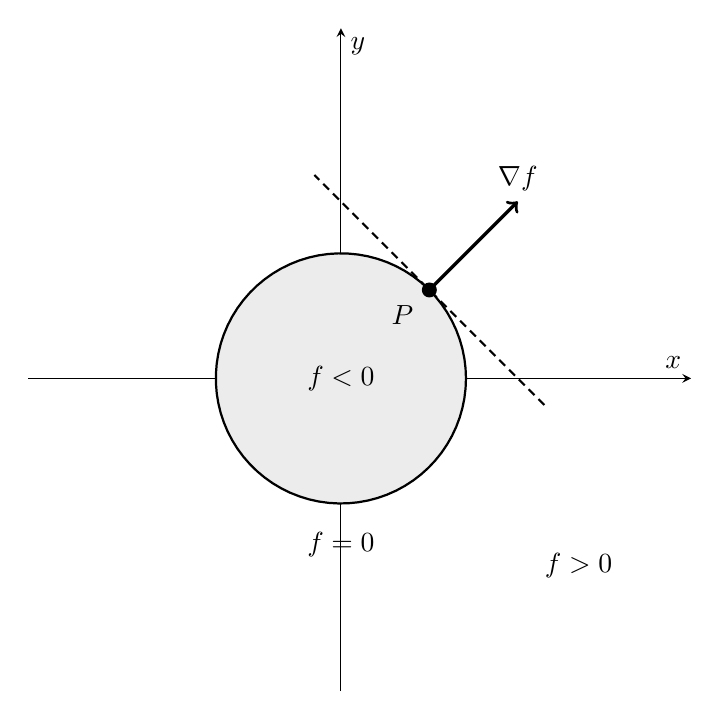
\begin{tikzpicture}
    \begin{axis}[
        width=10cm, height=10cm,
        xlabel=$x$, ylabel=$y$,
        axis lines=center, axis equal,
        xmin=-2.5, xmax=2.8, ymin=-2.5, ymax=2.8,
        ticks=none,
    ]
    % shaded interior f < 0
    \addplot[fill=gray!15, draw=none, domain=0:360, samples=80]
        ({cos(x)},{sin(x)}) \closedcycle;
    % level curve f = 0 (the unit circle)
    \addplot[thick, domain=0:360, samples=80]
        ({cos(x)},{sin(x)});
    \node at (axis cs:0,0) {$f<0$};
    \node at (axis cs:1.9,-1.5) {$f>0$};
    \node[below] at (axis cs:0,-1.15) {$f=0$};
    % point P = (1/sqrt2, 1/sqrt2) on the circle
    \addplot[only marks, mark=*, mark size=2.5pt]
        coordinates {({1/sqrt(2)},{1/sqrt(2)})};
    \node[below left] at (axis cs:{1/sqrt(2)-0.05},{1/sqrt(2)-0.05}) {$P$};
    % tangent line at P: direction (-1,1)
    \draw[thick, densely dashed]
        (axis cs:{1/sqrt(2)+1.3/sqrt(2)},{1/sqrt(2)-1.3/sqrt(2)})
        -- (axis cs:{1/sqrt(2)-1.3/sqrt(2)},{1/sqrt(2)+1.3/sqrt(2)});
    % normal vector nabla f at P, pointing outward
    \draw[->, very thick]
        (axis cs:{1/sqrt(2)},{1/sqrt(2)})
        -- (axis cs:{1/sqrt(2)+1/sqrt(2)},{1/sqrt(2)+1/sqrt(2)})
        node[above]{$\nabla f$};
    \end{axis}
\end{tikzpicture}
\end{center}

\begin{definition}[Tangent plane to a level surface]
Tangent plane to $f(x,y,z)=0$ at $P$ is
\[
    \nabla f(P)\cdot(\mathbf{x}-P)=0
\]
\end{definition}

\begin{example}
Find the tangent plane to $x^{3}+yz^{2}+4z=-5$ at $P=(1,-2,3)$.

Let $f(x,y,z)=x^{3}+yz^{2}+4z+5$, so $f(P)=0$.

$\nabla f(P)=\begin{pmatrix}3x^{2}\\z^{2}\\2yz+4\end{pmatrix}\bigg|_{P}
=\begin{pmatrix}3\\9\\-8\end{pmatrix}$

Tangent plane: $3(x-1)+9(y+2)-8(z-3)=0$
\end{example}

\begin{example}[Tangent plane to a cone]
$\left(\dfrac{x}{a}\right)^{2}+\left(\dfrac{y}{b}\right)^{2}=z^{2}$
at $P(x_{0},y_{0},z_{0})$.

Let $f=\left(\dfrac{x}{a}\right)^{2}+\left(\dfrac{y}{b}\right)^{2}-z^{2}$.
\[
    \nabla f(P)
    =\begin{pmatrix}2x_{0}/a^{2}\\2y_{0}/b^{2}\\-2z_{0}\end{pmatrix}
\]

Tangent plane: $\nabla f(P)\cdot(\mathbf{x}-P)=0$:
\[
    \frac{x_{0}x}{a^{2}}+\frac{y_{0}y}{b^{2}}=z_{0}z
\]
(using $(x_{0}/a)^{2}+(y_{0}/b)^{2}=z_{0}^{2}$ to cancel constants)
\end{example}

\begin{example}[Gradient ascent]
Suppose a mountain has height $z=f(x,y)$.
Climb as fast as possible: $\mathbf{r}'(t)\parallel\nabla f(\mathbf{r}(t))$.

\begin{center}
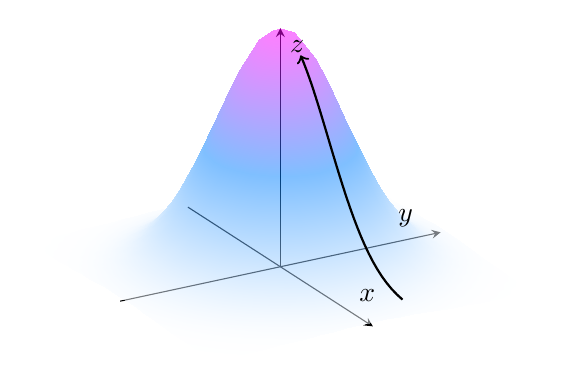
\begin{tikzpicture}
    \begin{axis}[
        view={60}{30}, width=8cm, height=7cm,
        xlabel=$x$, ylabel=$y$, zlabel=$z$,
        domain=-2:2, y domain=-2:2,
        samples=25, colormap/cool,
        axis lines=center, ticks=none,
    ]
    \addplot3[surf, opacity=0.5, shader=interp]{exp(-x^2-y^2)*2};
    % gradient ascent path projected on surface
    \addplot3[thick, ->, domain=0:1.8, samples=40, samples y=0]
        ({1.8*exp(-x)*cos(deg(0.3))},
         {1.8*exp(-x)*sin(deg(0.3))},
         {2*exp(-(1.8*exp(-x))^2)});
    \end{axis}
\end{tikzpicture}
\end{center}

\[
    \begin{pmatrix}x'(t)\\y'(t)\end{pmatrix}
    = \lambda\begin{pmatrix}f_{x}(\mathbf{r}(t))\\f_{y}(\mathbf{r}(t))\end{pmatrix}
    \;\Longleftrightarrow\;
    \frac{dy}{dx}=\frac{y'}{x'}=\frac{f_{y}}{f_{x}}
    \quad\text{(differential equation)}
\]
\end{example}

\subsection{Maximum and Minimum Values}

\begin{definition}[Local maximum]
$f(\mathbf{x})$, $\R^{n}\mapsto\R$. \;
$x=\xi$ is a local maximum if $f(\mathbf{y})\le f(\xi)$ for all $\mathbf{y}$ near $\xi$.

Formally: $\exists\,\delta>0$ such that
$\lvert\mathbf{y}-\xi\rvert<\delta \;\Longrightarrow\; f(\mathbf{y})\le f(\xi)$.
\end{definition}

Recall single variable: local max/min $\;\Longrightarrow\;$ $\nabla f(\xi)$ is $\mathbf{0}$ or DNE.

\begin{example}
$f(x,y)=7x-x^{2}-y^{2}$
\[
    = -(x-\tfrac{7}{2})^{2}+\tfrac{49}{4}-y^{2}
    \le \tfrac{49}{4} = f(\tfrac{7}{2},0)
\]
$\nabla f(\tfrac{7}{2},0) = \ldots = \mathbf{0}$.
\end{example}

Why? If $\nabla f(\xi)\neq\mathbf{0}$, say $f_{x}(\xi)>0$, then
for small $h>0$: $f(\xi+(h,0,\ldots))>f(\xi)$,
so we can take a small step to increase $f$ — $\xi$ is not a local max.
Vice versa, not min.

\begin{definition}[Critical point]
$f(\xi)$ is a critical point $\;\Longleftrightarrow\;$ $\nabla f(\xi)$
is either $\mathbf{0}$ or DNE.

Local max/min $\;\Longrightarrow\;$ critical point (but not conversely).
\end{definition}

\begin{definition}[Saddle point]
A critical point where the graph crosses its tangent plane.
\end{definition}

\begin{example}
$f(x,y)=x^{3}y^{2}$. \;
$\nabla f=\begin{pmatrix}3x^{2}y^{2}\\2x^{3}y\end{pmatrix}=\mathbf{0}$
gives infinite critical points: $(a,0)$ and $(0,b)$ for any $a,b$.

Consider $P=(0,1)$: nearby, $f(x,1)=x^{3}$ crosses the tangent line
$\;\Longrightarrow\;$ $P$ is a saddle point.
\end{example}

\subsubsection*{Multivariable Second Derivative Test}

\begin{theorem}[Second derivative test]
Suppose $f(x,y)$ has continuous second derivatives near
$\xi=(x_{0},y_{0})$ with $\nabla f(\xi)=\mathbf{0}$.
Define
\[
    D = f_{xx}(\xi)\,f_{yy}(\xi)-\bigl(f_{xy}(\xi)\bigr)^{2}
    = \det\begin{pmatrix}f_{xx}&f_{xy}\\f_{yx}&f_{yy}\end{pmatrix}
\]
\begin{enumerate}[nosep]
    \item $D>0$, $f_{xx}>0$: $\xi$ is a local minimum
    \item $D>0$, $f_{xx}<0$: $\xi$ is a local maximum
    \item $D<0$: $\xi$ is a saddle point
    \item $D=0$: no conclusion
\end{enumerate}
\end{theorem}

\begin{example}
$f(x,y)=(x^{2}+y^{2})e^{-x}$.
\[
    \nabla f
    = e^{-x}\begin{pmatrix}2x-x^{2}-y^{2}\\2y\end{pmatrix}
\]
Critical points: $\nabla f=\mathbf{0}$
\[
    \begin{cases}2x-x^{2}-y^{2}=0\\2y=0\end{cases}
    \;\Longleftrightarrow\;
    y=0,\; x=0\text{ or }2
\]
Two critical points: $(0,0)$ and $(2,0)$.

$D = f_{xx}f_{yy}-(f_{xy})^{2}$

At $(0,0)$: $D=4>0$, $f_{xx}=2>0$ $\;\Longrightarrow\;$ minimum.

At $(2,0)$: $D=-4e^{-4}<0$ $\;\Longrightarrow\;$ saddle.
\end{example}

\begin{example}
$f(x,y)=11x^{2}-2xy+2y^{2}+3y$. Identify critical points.

$\nabla f = \begin{pmatrix}22x-2y\\-2x+4y+3\end{pmatrix}$

Let $\nabla f=\mathbf{0}$:
$\begin{cases}22x-2y=0\\-2x+4y+3=0\end{cases}
\;\Longrightarrow\;
x=-\tfrac{1}{14},\; y=-\tfrac{11}{14}$

Only one critical point.

$D = \begin{vmatrix}f_{xx}&f_{xy}\\f_{yx}&f_{yy}\end{vmatrix}
= \begin{vmatrix}22&-2\\-2&4\end{vmatrix}
= 84>0$

$D>0$, $f_{xx}>0$ $\;\Longrightarrow\;$ minimum.
\end{example}

\begin{example}[Minimum distance from a surface to a point]
Minimize the distance from a point on $z=x^{2}+y$ to $(2,0,0)$.

$\text{dist}^{2} = f^{2}(x,y) = (x-2)^{2}+y^{2}+z^{2}
= (x-2)^{2}+y^{2}+(x^{2}+y)^{2}$

\[
    \nabla(f^{2})
    = \begin{pmatrix}2(x-2)+4x(x^{2}+y)\\2y+2(x^{2}+y)\end{pmatrix}
\]

$\nabla(f^{2})=\mathbf{0}$: from the second component, $y=-\tfrac{1}{2}x^{2}$.
Substituting into the first:
\[
    x^{3}+x-2 = 0
    \;\Longrightarrow\;
    (x-1)(x^{2}+x+2)=0
\]
$x=1$ is the only real root. $y=-\tfrac{1}{2}$.

Only one critical point $(1,-\tfrac{1}{2})$,
on the cylinder at $(1,-\tfrac{1}{2},\tfrac{1}{2})$.
\end{example}

\begin{example}[Maximize a product with a constraint]
Maximize $xyz$ subject to $x+y+z=12$.

$f(x,y) = xy(12-x-y)$

$\nabla f = \begin{pmatrix}12y-2xy-y^{2}\\12x-x^{2}-2xy\end{pmatrix}$

Let $\nabla f=\mathbf{0}$:
$\begin{cases}12y-2xy-y^{2}=0\\12x-x^{2}-2xy=0\end{cases}$

Since we want to maximize $xyz>0$, ignore critical points with
$x=0$ or $y=0$. The remaining solution is $(4,4)$, giving $z=4$.

$D(4,4) = \begin{vmatrix}-8&-4\\-4&-8\end{vmatrix} > 0$, \;
$f_{xx}<0$ $\;\Longrightarrow\;$ maximum.
\end{example}

\subsection{Lagrange Multipliers}

Want to solve $\max/\min\; f(\mathbf{x})$ subject to $g(\mathbf{x})=0$.
Useful when it is hard to substitute the constraint $g(\mathbf{x})=0$ directly.

\textbf{Idea.}
Consider $f(x,y)=xy$, $g(x,y)=x+y-12$.
At the constrained max/min, the level curve of $f$ is tangent to the
constraint $g=0$, so $\nabla f\parallel\nabla g$.

\begin{center}
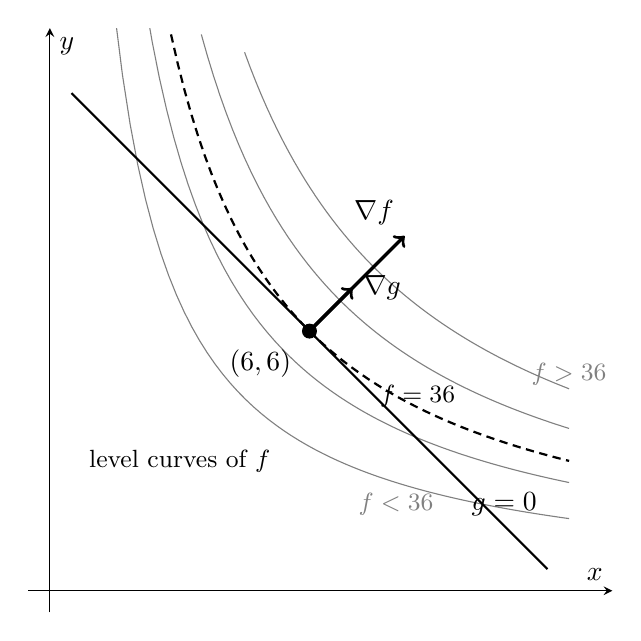
\begin{tikzpicture}
    \begin{axis}[
        width=9cm, height=9cm,
        xlabel=$x$, ylabel=$y$,
        axis lines=center,
        ticks=none,
        xmin=-0.5, xmax=13, ymin=-0.5, ymax=13,
    ]
    % level curves of f = xy (f < 0 not possible for xy in first quadrant)
    % f < 36: below tangent curve
    \addplot[thin, gray, domain=1.5:12, samples=60]{20/x};
    \addplot[thin, gray, domain=2.2:12, samples=60]{30/x};
    % f = 36: tangent to constraint
    \addplot[thick, densely dashed, domain=2.8:12, samples=60]{36/x};
    % f > 36
    \addplot[thin, gray, domain=3.5:12, samples=60]{45/x};
    \addplot[thin, gray, domain=4.5:12, samples=60]{56/x};
    % labels
    \node at (axis cs:3,3) {\small level curves of $f$};
    \node[gray] at (axis cs:8,2) {\small$f<36$};
    \node at (axis cs:8.5,4.5) {\small$f=36$};
    \node[gray] at (axis cs:12,5) {\small$f>36$};
    % constraint g = 0: x + y = 12
    \addplot[thick, domain=0.5:11.5]{12-x};
    \node at (axis cs:10.5,2) {$g=0$};
    % tangent point (6,6)
    \addplot[only marks, mark=*, mark size=2.5pt] coordinates {(6,6)};
    \node[below left] at (axis cs:5.8,5.8) {$(6,6)$};
    % nabla f = (y,x) = (6,6), nabla g = (1,1)
    % both point in direction (1,1) — show nabla f longer
    \draw[->, very thick] (axis cs:6,6) -- (axis cs:8.2,8.2)
        node[above left]{$\nabla f$};
    \draw[->, very thick] (axis cs:6,6) -- (axis cs:7,7)
        node[right]{$\nabla g$};
    \end{axis}
\end{tikzpicture}
\end{center}

At max, $\nabla f\parallel\nabla g$.

\subsubsection*{Lagrange Multiplier Method}

To solve $\max/\min\; f(\mathbf{x})$ subject to $g(\mathbf{x})=k$:
\[
    \text{solve}\quad
    \begin{cases}\nabla f = \lambda\,\nabla g \\ g = k\end{cases}
\]
Solutions are candidates --- may be max, min, or saddle.

\begin{remark}
If $g(\mathbf{x})=0$ has corners or endpoints,
the Lagrange method may miss extreme there.
\end{remark}

\begin{theorem}[Extreme Value Theorem]
Suppose $f\colon D\to\R$ is continuous on a closed, bounded $D$.
\begin{enumerate}[nosep]
    \item Find critical points in $D$ by $\nabla f=\mathbf{0}$ in $D$.
    \item Find max/min on the boundary $\partial D$.
\end{enumerate}
The absolute max/min is among (1) and (2).
\end{theorem}

\begin{example}[Extreme Value Theorem on a square]
Find the absolute max/min of $f(x,y)=2x+y-3xy$ on $0\le x,y\le 1$.

\begin{center}
\begin{tikzpicture}
    \draw (0,0) rectangle (2,2);
    \node[below left] at (0,0) {$0$};
    \node[below] at (2,0) {$1$};
    \node[left] at (0,2) {$1$};
    \draw[->] (-0.3,0) -- (2.5,0) node[right]{$x$};
    \draw[->] (0,-0.3) -- (0,2.5) node[above]{$y$};
    \fill (0.67,1.33) circle(1.5pt) node[right]{\small$P$};
\end{tikzpicture}
\end{center}

\textbf{1. Interior critical point.}
$\nabla f = \begin{pmatrix}2-3y\\1-3x\end{pmatrix} = \mathbf{0}$
$\;\Longrightarrow\; x=\tfrac{1}{3},\; y=\tfrac{2}{3}$.
\; $f(\tfrac{1}{3},\tfrac{2}{3})=\tfrac{2}{3}$.

\textbf{2. Four edges.}
\begin{enumerate}[nosep]
    \item $x=0$: $f(0,y)=y$. \; max $=f(0,1)=1$, min $=f(0,0)=0$.
    \item $y=0$: $f(x,0)=2x$. \; max $=f(1,0)=2$, min $=f(0,0)=0$.
    \item $x=1$: $f(1,y)=2+y-3y=2-2y$. \; max $=f(1,0)=2$, min $=f(1,1)=0$.
    \item $y=1$: $f(x,1)=2x+1-3x=1-x$. \; max $=f(0,1)=1$, min $=f(1,1)=0$.
\end{enumerate}

Absolute max $=f(1,0)=2$. \;
Absolute min $=f(0,0)=f(1,1)=0$.
\end{example}

\begin{example}[Lagrange multiplier on a circle]
Minimize $f(x,y)=\sqrt{x^{2}+y^{2}}$ subject to $g(x,y)=2x+3y=6$.

$\nabla f = \lambda\,\nabla g$:
\[
    \frac{1}{\sqrt{x^{2}+y^{2}}}\begin{pmatrix}x\\y\end{pmatrix}
    = \lambda\begin{pmatrix}2\\3\end{pmatrix}
\]

\[
    \begin{cases}
        \dfrac{x}{\sqrt{x^{2}+y^{2}}} = 2\lambda \\[6pt]
        \dfrac{y}{\sqrt{x^{2}+y^{2}}} = 3\lambda \\[6pt]
        2x+3y = 6
    \end{cases}
\]

Dividing the first two equations: $\dfrac{x}{y}=\dfrac{2}{3}$
$\;\Longrightarrow\; x=\dfrac{12}{13},\; y=\dfrac{18}{13}$.

Only one critical point --- by the geometry (distance from origin to a line),
it is a minimum.

\begin{center}
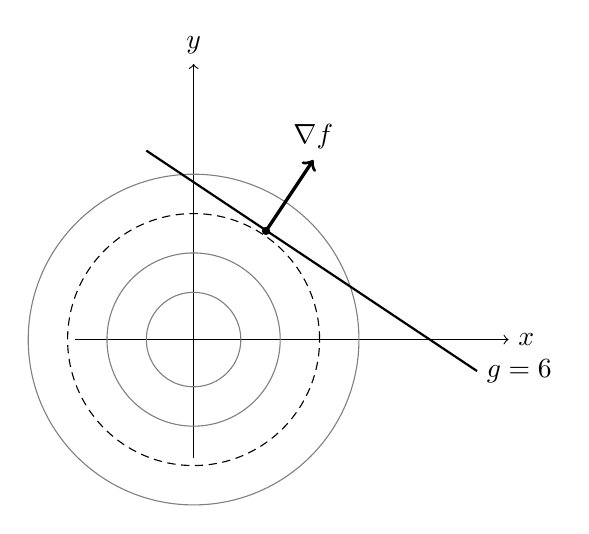
\begin{tikzpicture}
    \draw[->] (-1.5,0) -- (4,0) node[right]{$x$};
    \draw[->] (0,-1.5) -- (0,3.5) node[above]{$y$};
    % level curves of f (concentric circles)
    \draw[thin, gray] (0,0) circle(0.6);
    \draw[thin, gray] (0,0) circle(1.1);
    \draw[thin, densely dashed] (0,0) circle(1.6);
    \draw[thin, gray] (0,0) circle(2.1);
    % constraint line 2x + 3y = 6
    \draw[thick] (-0.6,2.4) -- (3.6,-0.4);
    \node[right] at (3.6,-0.4) {$g=6$};
    % closest point P = (12/13, 18/13) ≈ (0.92, 1.38)
    \fill (0.92,1.38) circle(1.5pt);
    % nabla f at P pointing from origin
    \draw[->, very thick] (0.92,1.38) -- (0.92+0.6,1.38+0.9)
        node[above]{$\nabla f$};
\end{tikzpicture}
\end{center}

\end{example}